\documentclass[fontsize=10pt]{scrartcl}

\usepackage{enumitem}
	\setenumerate{listparindent=\parindent}
\usepackage{amsmath}
\usepackage{amssymb}
\usepackage{graphicx}
\usepackage{placeins}
\usepackage{hyperref}
\usepackage{float}

\usepackage[margin=1.0in]{geometry}

\newcommand{\code}{\texttt}

\begin{document}

	\title{CSC 522 : Automated Learning and Data Analysis}
	\subtitle{Homework 2}
	\author{Roopak Venkatakrishnan - rvenkat7@ncsu.edu}
	\maketitle

	\section{Question 1}
		Write code in R or Matlab to perform each of the following tasks:
		\begin{enumerate}
			\item
			Generate a $3 \times 3$ matrix with input containing the sequence 1, 2, ... 9. \\
			\textbf{Ans:} $x \leftarrow matrix(c(1:9),3,3)$
			\item
			\begin{enumerate}
				\item
				Access elements from the 2nd and 3rd columns only. \\
				\textbf{Ans:} \\
				2nd column alone : x[,2] $\implies$ [1] 4 5 6\\
				3rd column alone : x[,3] $\implies$ [1] 7 8 9\\ 
				both columns     : x[,2:3] \\
				$\implies$ \\
				
				$\begin{array}{ccc} 
					~		&	[,1]	&	[,2]	\\ \relax
					[1,]	&	4	 	&	7		\\ \relax
					[2,]	&	5		&	8		\\ \relax
					[3,]	&	6		&	9		\\ \relax
				\end{array}$

				
				\item
				Access elements of the 2nd and 3rd rows only \\
				\textbf{Ans:} \\
				2nd row alone : x[2,] $\implies$ [1] 2 5 8\\
				3rd row alone : x[3,] $\implies$ [1] 3 6 9\\ 
				both rows     : x[2:3,] \\
				$\implies$ \\
				$\begin{array}{cccc}
					~		&	[,1]	&	[,2]	&	[,3]	\\ \relax
					[1,]	&	2		&	5		&	8		\\ \relax
					[2,]	&	3		&	6		&	9		\\ \relax
				\end{array}$


				\item
				Access rows 1 and 3 only? (see rbind() function in R and vertcat() in matlab) \\
				\textbf{Ans:} \\
				$x2 \leftarrow rbind(x[2,],x[3,])$ \\
				$\implies$ \\
				$\begin{array}{cccc}
					~		&	[,1]	&	[,2]	&	[,3]	\\ \relax
					[1,]	&	1		&	4		&	7		\\ \relax
					[2,]	&	3		&	6		&	9		\\ \relax
				\end{array}$

				\item
				Calculate sum of the 2nd row, the diagonal and the 3rd column in the matrix. \\
				\textbf{Ans:} \\
				x[2,] + x[,3] + diag(x) \\
				$\implies$  [1] 10 18 26 \\

				\item
				Identify row and column dimensions of the matrix.\\
				\textbf{Ans:} \\
				dim(x) \\
				$\implies$ [1] 3 3 \\

				\item
				Transpose of a matrix. \\
				\textbf{Ans:} \\
				t(x) \\
				$\begin{array}{cccc}
				~		&	[,1]	&	[,2]	&	[,3]	\\ \relax
				[1,]	&	1		&	2		&	3		\\ \relax
				[2,]	&	4		&	5		&	6		\\ \relax
				[3,]	&	7		&	8		&	9		\\ \relax
				\end{array}$

				\item
				Scalar multiplication of output matrix with itself. \\
				\textbf{Ans:} \\
				x * x \\
				$\begin{array}{cccc}
				~		&	[,1]	&	[,2]	&	[,3]	\\ \relax
				[1,]	&	1		&	16		&	49		\\ \relax
				[2,]	&	4		&	25		&	64		\\ \relax
				[3,]	&	9		&	36		&	81		\\ \relax
				\end{array}$

				\item
				Matrix multiplication of output matrix with itself. \\
				\textbf{Ans:} \\
				x \%*\% x \\
				$\begin{array}{cccc}
				~		&	[,1]	&	[,2]	&	[,3]	\\ \relax
				[1,]	&	30		&	66		&	102		\\ \relax
				[2,]	&	36		&	81		&	126		\\ \relax
				[3,]	&	42		&	96		&	150		\\ \relax
				\end{array}$

				\item
				Cross product of the output matrix from 1. \\
				\textbf{Ans:} \\
				crossprod(x) \\
				$\begin{array}{cccc}
				~		&	[,1]	&	[,2]	&	[,3]	\\ \relax
				[1,]	&	14		&	32		&	50		\\ \relax
				[2,]	&	32		&	77		&	122		\\ \relax
				[3,]	&	50		&	122		&	194		\\ \relax
				\end{array}$

				\item
				Check if a matrix is a square matrix. \\
				\textbf{Ans:} \\
				\begin{verbatim}
function checksqmatrix(mat) 
{ 
  if(dim(mat)[1]==dim(mat)[2]) 
  { 
    print("It is a square matrix!") 
  } 
  else 
  { 
    print("It is NOT a square matrix") 
  } 
} 

> checksqmatrix(x)
[1] "It is a square matrix!"

> checksqmatrix(matrix(c(1:10),2,5))
[1] "It is NOT a square matrix"
\end{verbatim}
				
				\item
				Inverse of a matrix \\
				\textbf{Ans:} \\
				solve(x) \\
				Since this matrix has determinant 0 the inverse is not defined. \\
				Error in solve.default(x) :  \\
  				Lapack routine dgesv: system is exactly singular: U[3,3] = 0 \\

  				\item
  				Identity of a matrix. \\
  				\textbf{Ans:} \\

  				\item
  				Sum of all elements in the matrix (use a for/while loop) \\
\begin{verbatim}
matrixsum <- function (mat) {
  i<-1
  sum<-0
  while(i<=dim(mat)[1]*dim(mat)[2])
  {
    sum<-sum+mat[i]
    i<-i+1
  }
  print (paste(sum, "is the sum of elements"))
}

> matrixsum(x)
[1] "45 is the sum of elements"
\end{verbatim}

			\end{enumerate}
		\end{enumerate}

	\section{Question 2}
	For this exercise, use the “values.txt” file provided. The file contains a list of 150 data instances. There are 2 columns representing the x and y coordinates. Complete the following tasks: \\
	\begin{enumerate}
		\item
		Load the file
		\textbf{Ans:} \\
		$\implies$
		vals = read.table("D:
		\textbackslash\textbackslash
		Courses
		\textbackslash\textbackslash
		datamining - CSC522
		\textbackslash\textbackslash
		homework
		\textbackslash\textbackslash
		hw2
		\textbackslash\textbackslash
		values.txt")

		\item
		Make a 2-D plot and label the axes \\
		plot(vals,main="A 2D plot of values.txt",xlab="Values of V1",ylab="Values of V2") \\
		\begin{figure}[H]
			\begin{center}
				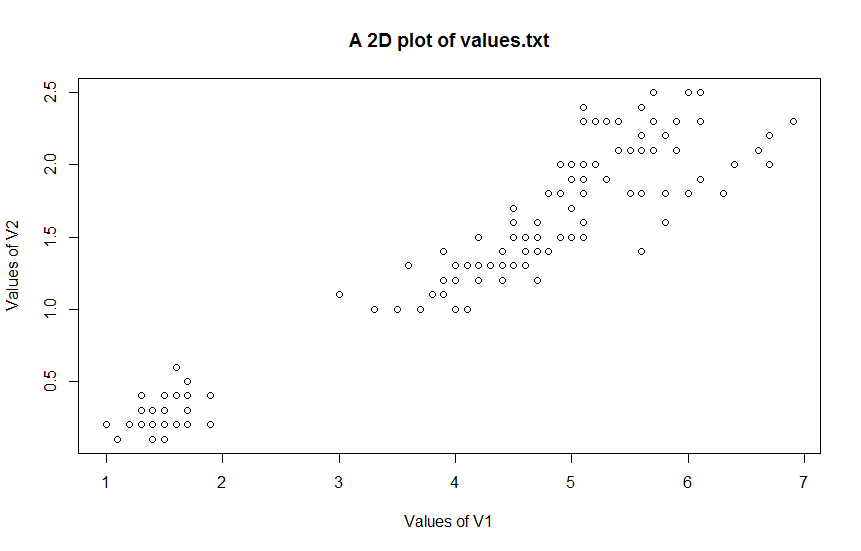
\includegraphics[scale=.5]{resources/q2_plot.png}
				\caption{The 2D plot obtained from values.txt}
			\end{center}
		\end{figure}

		\item
		Find the correlation between the dimensions. \\
		cor(vals) \\
		$\begin{array}{ccc}
			~		&		V1			&	V2			\\
			V1 		&		1.0000000	&	0.9628654	\\
			V2		&		0.9628654	&	1.0000000	\\
		\end{array}$

		\item
		Now consider a point (5; 1:5).
			\begin{enumerate}
				\item
				Compute the distance of this point from each of the 150 instances using Euclidean distance, Mahalanobis distance, City block metric, Minkowski metric, Chebychev distance and Cosine distance. \\
				\textbf{Ans:} \\

				\textbf{\large Euclidean Distance} \\
\begin{verbatim}
library(fields)
rdist(vals,matrix(c(5,1.5),1,2))
             [,1]
  [1,] 3.8275318418
  [2,] 3.8275318418
  [3,] 3.9217343102
  [4,] 3.7336309405
  [5,] 3.8275318418
  [6,] 3.4785054262
  [7,] 3.7947331922
  [8,] 3.7336309405
  [9,] 3.8275318418
 [10,] 3.7696153650
 [11,] 3.7336309405
 [12,] 3.6400549446
 [13,] 3.8626415832
 [14,] 4.1436698710
 [15,] 4.0162171256
 [16,] 3.6687872656
 [17,] 3.8600518131
 [18,] 3.7947331922
 [19,] 3.5114099732
 [20,] 3.7000000000
 [21,] 3.5468295702
 [22,] 3.6687872656
 [23,] 4.2059481690
 [24,] 3.4481879299
 [25,] 3.3615472628
 [26,] 3.6400549446
 [27,] 3.5735136770
 [28,] 3.7336309405
 [29,] 3.8275318418
 [30,] 3.6400549446
 [31,] 3.6400549446
 [32,] 3.6687872656
 [33,] 3.7696153650
 [34,] 3.8275318418
 [35,] 3.7336309405
 [36,] 4.0162171256
 [37,] 3.9217343102
 [38,] 3.8626415832
 [39,] 3.9217343102
 [40,] 3.7336309405
 [41,] 3.8897300678
 [42,] 3.8897300678
 [43,] 3.9217343102
 [44,] 3.5171010790
 [45,] 3.2893768407
 [46,] 3.7947331922
 [47,] 3.6400549446
 [48,] 3.8275318418
 [49,] 3.7336309405
 [50,] 3.8275318418
 [51,] 0.3162277660
 [52,] 0.5000000000
 [53,] 0.1000000000
 [54,] 1.0198039027
 [55,] 0.4000000000
 [56,] 0.5385164807
 [57,] 0.3162277660
 [58,] 1.7720045147
 [59,] 0.4472135955
 [60,] 1.1045361017
 [61,] 1.5811388301
 [62,] 0.8000000000
 [63,] 1.1180339887
 [64,] 0.3162277660
 [65,] 1.4142135624
 [66,] 0.6082762530
 [67,] 0.5000000000
 [68,] 1.0295630141
 [69,] 0.5000000000
 [70,] 1.1704699911
 [71,] 0.3605551275
 [72,] 1.0198039027
 [73,] 0.1000000000
 [74,] 0.4242640687
 [75,] 0.7280109889
 [76,] 0.6082762530
 [77,] 0.2236067977
 [78,] 0.2000000000
 [79,] 0.5000000000
 [80,] 1.5811388301
 [81,] 1.2649110641
 [82,] 1.3928388277
 [83,] 1.1401754251
 [84,] 0.1414213562
 [85,] 0.5000000000
 [86,] 0.5099019514
 [87,] 0.3000000000
 [88,] 0.6324555320
 [89,] 0.9219544457
 [90,] 1.0198039027
 [91,] 0.6708203932
 [92,] 0.4123105626
 [93,] 1.0440306509
 [94,] 1.7720045147
 [95,] 0.8246211251
 [96,] 0.8544003745
 [97,] 0.8246211251
 [98,] 0.7280109889
 [99,] 2.0396078054
[100,] 0.9219544457
[101,] 1.4142135624
[102,] 0.4123105626
[103,] 1.0816653826
[104,] 0.6708203932
[105,] 1.0630145813
[106,] 1.7088007491
[107,] 0.5385164807
[108,] 1.3341664064
[109,] 0.8544003745
[110,] 1.4866068747
[111,] 0.5099019514
[112,] 0.5000000000
[113,] 0.7810249676
[114,] 0.5000000000
[115,] 0.9055385138
[116,] 0.8544003745
[117,] 0.5830951895
[118,] 1.8384776311
[119,] 2.0615528128
[120,] 0.0000000001
[121,] 1.0630145813
[122,] 0.5099019514
[123,] 1.7720045147
[124,] 0.3162277660
[125,] 0.9219544457
[126,] 1.0440306509
[127,] 0.3605551275
[128,] 0.3162277660
[129,] 0.8485281374
[130,] 0.8062257748
[131,] 1.1704699911
[132,] 1.4866068747
[133,] 0.9219544457
[134,] 0.1000000000
[135,] 0.6082762530
[136,] 1.3601470509
[137,] 1.0816653826
[138,] 0.5830951895
[139,] 0.3605551275
[140,] 0.7211102551
[141,] 1.0816653826
[142,] 0.8062257748
[143,] 0.4123105626
[144,] 1.2041594579
[145,] 1.2206555616
[146,] 0.8246211251
[147,] 0.4000000000
[148,] 0.5385164807
[149,] 0.8944271910
[150,] 0.3162277660


\end{verbatim}

				\textbf{\large Manhatten Distance} \\

\begin{verbatim}
> abs(vals[["V2"]]-1.5) + abs(vals[["V1"]]-5)
  [1] 4.9 4.9 5.0 4.8 4.9 4.4 4.8 4.8 4.9 4.9 4.8 4.7
 [13] 5.0 5.3 5.1 4.6 4.8 4.8 4.5 4.7 4.6 4.6 5.3 4.3
 [25] 4.4 4.7 4.5 4.8 4.9 4.7 4.7 4.6 4.9 4.9 4.8 5.1
 [37] 5.0 5.0 5.0 4.8 4.9 4.9 5.0 4.3 4.2 4.8 4.7 4.9
 [49] 4.8 4.9 0.4 0.5 0.1 1.2 0.4 0.7 0.4 2.2 0.6 1.2
 [61] 2.0 0.8 1.5 0.4 1.6 0.7 0.5 1.4 0.5 1.5 0.5 1.2
 [73] 0.1 0.6 0.9 0.7 0.3 0.2 0.5 2.0 1.6 1.8 1.4 0.2
 [85] 0.5 0.6 0.3 0.8 1.1 1.2 0.9 0.5 1.3 2.2 1.0 1.1
 [97] 1.0 0.9 2.4 1.1 2.0 0.5 1.5 0.9 1.5 2.2 0.7 1.6
[109] 1.1 2.1 0.6 0.7 1.1 0.5 1.0 1.1 0.8 2.4 2.7 0.0
[121] 1.5 0.6 2.2 0.4 1.3 1.3 0.5 0.4 1.2 0.9 1.5 1.9
[133] 1.3 0.1 0.7 1.9 1.5 0.8 0.5 1.0 1.5 0.9 0.5 1.7
[145] 1.7 1.0 0.4 0.7 1.2 0.4


\end{verbatim}

			\textbf{\large Cosine Distance} \\
\begin{verbatim}
> cosnum <- vals[["V1"]]*5 + vals[["V2"]]*1.5
> cosden<- sqrt(27.25) * sqrt((vals[["V1"]]*vals[["V1"]]) 
+                             + (vals[["V2"]]*vals[["V2"]]))
> cosdist <- cosnum/cosden
> cosdist
  [1] 0.9888368 0.9888368 0.9903817 0.9874011 0.9888368 0.9981785 0.9967726
  [8] 0.9874011 0.9888368 0.9748189 0.9874011 0.9860710 0.9758649 0.9799079
 [15] 0.9920337 0.9995240 0.9999752 0.9967726 0.9931884 0.9955795 0.9848398
 [22] 0.9995240 0.9955795 0.9999854 0.9826444 0.9860710 0.9989201 0.9874011
 [29] 0.9888368 0.9860710 0.9860710 0.9995240 0.9748189 0.9888368 0.9874011
 [36] 0.9920337 0.9903817 0.9758649 0.9903817 0.9874011 0.9979104 0.9979104
 [43] 0.9903817 0.9977353 0.9964774 0.9967726 0.9860710 0.9888368 0.9874011
 [50] 0.9888368 0.9999981 0.9995412 0.9999843 0.9997407 0.9997178 0.9999477
 [57] 0.9993280 0.9999961 0.9998715 0.9985857 0.9999134 0.9986707 0.9989201
 [64] 0.9999981 0.9984834 0.9998623 0.9995412 0.9986366 0.9995412 0.9998631
 [71] 0.9977353 0.9997407 0.9999843 0.9991399 0.9999977 0.9998623 0.9999706
 [78] 0.9993419 0.9995412 0.9999134 0.9999531 0.9996221 0.9999752 0.9999213
 [85] 0.9995412 0.9987423 0.9998473 0.9999913 0.9998785 0.9997407 0.9996824
 [92] 0.9999921 1.0000000 0.9999961 0.9999620 0.9999134 0.9999620 0.9999977
 [99] 0.9982013 0.9998785 0.9946658 0.9978776 0.9987255 0.9998091 0.9974744
[106] 0.9998623 0.9975687 0.9999134 0.9999552 0.9952506 0.9966177 0.9986084
[113] 0.9973164 0.9960377 0.9890110 0.9930484 0.9996918 0.9996670 0.9995412
[120] 1.0000000 0.9957645 0.9953891 0.9999991 0.9981651 0.9981074 1.0000000
[127] 0.9977353 0.9981651 0.9977353 0.9997516 0.9999449 0.9999347 0.9965677
[134] 0.9999854 0.9989201 0.9976129 0.9935731 0.9996918 0.9977353 0.9968467
[141] 0.9935731 0.9912727 0.9978776 0.9967815 0.9925826 0.9921999 0.9974314
[148] 0.9971348 0.9938239 0.9988561


\end{verbatim}
			
			\textbf{\large Chebyshev Distance} \\

\begin{verbatim}
> v4<-cbind(abs(vals$V1-5),abs(vals$V2-1.5))
> tchebyshev <- sapply(v4,max)
> tchebyshev
  [1] 3.6 3.6 3.7 3.5 3.6 3.3 3.6 3.5 3.6 3.5 3.5 3.4 3.6 3.9 3.8
 [16] 3.5 3.7 3.6 3.3 3.5 3.3 3.5 4.0 3.3 3.1 3.4 3.4 3.5 3.6 3.4
 [31] 3.4 3.5 3.5 3.6 3.5 3.8 3.7 3.6 3.7 3.5 3.7 3.7 3.7 3.4 3.1
 [46] 3.6 3.4 3.6 3.5 3.6 0.3 0.5 0.1 1.0 0.4 0.5 0.3 1.7 0.4 1.1
 [61] 1.5 0.8 1.0 0.3 1.4 0.6 0.5 0.9 0.5 1.1 0.2 1.0 0.1 0.3 0.7
 [76] 0.6 0.2 0.0 0.5 1.5 1.2 1.3 1.1 0.1 0.5 0.5 0.3 0.6 0.9 1.0
 [91] 0.6 0.4 1.0 1.7 0.8 0.8 0.8 0.7 2.0 0.9 1.0 0.1 0.9 0.6 0.8
[106] 1.6 0.5 1.3 0.8 1.1 0.1 0.3 0.5 0.0 0.1 0.3 0.5 1.7 1.9 0.0
[121] 0.7 0.1 1.7 0.1 0.7 1.0 0.2 0.1 0.6 0.8 1.1 1.4 0.6 0.1 0.6
[136] 1.1 0.6 0.5 0.2 0.4 0.6 0.1 0.1 0.9 0.7 0.2 0.0 0.2 0.4 0.1
[151] 1.3 1.3 1.3 1.3 1.3 1.1 1.2 1.3 1.3 1.4 1.3 1.3 1.4 1.4 1.3
[166] 1.1 1.1 1.2 1.2 1.2 1.3 1.1 1.3 1.0 1.3 1.3 1.1 1.3 1.3 1.3
[181] 1.3 1.1 1.4 1.3 1.3 1.3 1.3 1.4 1.3 1.3 1.2 1.2 1.3 0.9 1.1
[196] 1.2 1.3 1.3 1.3 1.3 0.1 0.0 0.0 0.2 0.0 0.2 0.1 0.5 0.2 0.1
[211] 0.5 0.0 0.5 0.1 0.2 0.1 0.0 0.5 0.0 0.4 0.3 0.2 0.0 0.3 0.2
[226] 0.1 0.1 0.2 0.0 0.5 0.4 0.5 0.3 0.1 0.0 0.1 0.0 0.2 0.2 0.2
[241] 0.3 0.1 0.3 0.5 0.2 0.3 0.2 0.2 0.4 0.2 1.0 0.4 0.6 0.3 0.7
[256] 0.6 0.2 0.3 0.3 1.0 0.5 0.4 0.6 0.5 0.9 0.8 0.3 0.7 0.8 0.0
[271] 0.8 0.5 0.5 0.3 0.6 0.3 0.3 0.3 0.6 0.1 0.4 0.5 0.7 0.0 0.1
[286] 0.8 0.9 0.3 0.3 0.6 0.9 0.8 0.4 0.8 1.0 0.8 0.4 0.5 0.8 0.3


\end{verbatim}
			\textbf{\large Minkowski Distance(p=3)} \\

\begin{verbatim}
> vals2 <- cbind(abs(vals$V1-5),abs(vals$V2-1.5))
> minkowski <- (vals2[,1]^3 + vals2[,2]^3)^(1/3)
> minkowski
  [1] 3.6556427 3.6556427 3.7527387 3.5587893 3.6556427
  [6] 3.3402479 3.6439068 3.5587893 3.6556427 3.5731281
 [11] 3.5587893 3.4622056 3.6692360 3.9592317 3.8500534
 [16] 3.5358492 3.7321283 3.6439068 3.3520667 3.5464025
 [21] 3.3659226 3.5358492 4.0452569 3.3303295 3.1744052
 [26] 3.4622056 3.4379542 3.5587893 3.6556427 3.4622056
 [31] 3.4622056 3.5358492 3.5731281 3.6556427 3.5587893
 [36] 3.8500534 3.7527387 3.6692360 3.7527387 3.5587893
 [41] 3.7416049 3.7416049 3.7527387 3.4208921 3.1454962
 [46] 3.6439068 3.4622056 3.6556427 3.5587893 3.6556427
 [51] 0.3036589 0.5000000 0.1000000 1.0026596 0.4000000
 [56] 0.5104469 0.3036589 1.7142970 0.4160168 1.1002754
 [61] 1.5182945 0.8000000 1.0400419 0.3036589 1.4013592
 [66] 0.6009245 0.5000000 0.9487518 0.5000000 1.1173556
 [71] 0.3271066 1.0026596 0.1000000 0.3779763 0.7054004
 [76] 0.6009245 0.2080084 0.2000000 0.5000000 1.5182945
 [81] 1.2146356 1.3242015 1.1073883 0.1259921 0.5000000
 [86] 0.5013298 0.3000000 0.6073178 0.9032802 1.0026596
 [91] 0.6240251 0.4020726 1.0089202 1.7142970 0.8041452
 [96] 0.8138223 0.8041452 0.7054004 2.0053192 0.9032802
[101] 1.2599210 0.4020726 0.9813199 0.6240251 0.9491220
[106] 1.6276446 0.5104469 1.3053038 0.8138223 1.3259101
[111] 0.5013298 0.4497941 0.6986368 0.5000000 0.9004113
[116] 0.8138223 0.5336803 1.7386752 1.9461462 0.0000000
[121] 0.9491220 0.5013298 1.7142970 0.3036589 0.8237661
[126] 1.0089202 0.3271066 0.3036589 0.7559526 0.8005205
[131] 1.1173556 1.4209436 0.8237661 0.1000000 0.6009245
[136] 1.2260507 0.9813199 0.5336803 0.3271066 0.6542133
[141] 0.9813199 0.8005205 0.4020726 1.0746258 1.1032959
[146] 0.8041452 0.4000000 0.5104469 0.8320335 0.3036589


\end{verbatim}
\newpage
				\item
				For each distance measure, identify the 10 points from the dataset that are the closest to the point(5,1.5).
				\begin{itemize}
					\item
					Create plots, one for each distance measure. Place an ‘X’ for (5,1.5) and mark the 10 closest points. To mark them, you could place a circle or any other shape over the point.

					\item
					Verify if the set of points is the same across all the distance measures.
				\end{itemize}
				. \\
				. \\
				\textbf{\large Minkowski Distance(p=3)} \\
\begin{verbatim}
> mink2 <- cbind(vals,minkowski)
> mink3<-head(mink2[order(minkowski),],10)
> plot(mink3[["V1"]],mink3[["V2"]],xlab="V1",ylab="V2",
+							main="Graph for Minkowski Distance",xlim=c(4.5,5.5),ylim=c(1.35,1.8))
> points(5,1.5,type="b",pch=4,col="#660000",cex=3)
\end{verbatim}
			\begin{figure}[H]
				\begin{center}
					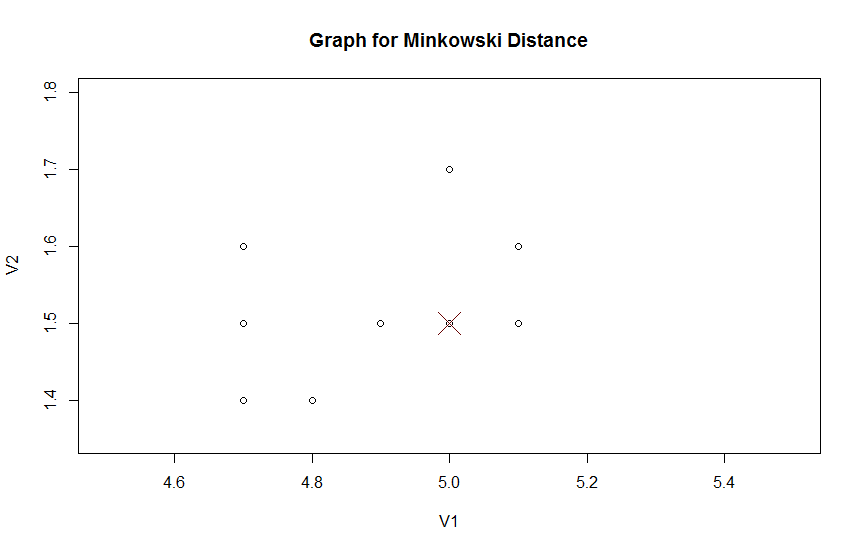
\includegraphics[scale=.5]{resources/minkowski.png}
					\caption{The plot for Minkowski Distance}
				\end{center}
			\end{figure}

			\newpage
			\textbf{\large Tchebyshev Distance} \\

\begin{verbatim}
> tcheby1 <- cbind(vals,tchebyshev)
> tcheby2<-head(tcheby1[order(tchebyshev),],10)
> plot(tcheby2[["V1"]],tcheby2[["V2"]],xlab="V1",ylab="V2"
+								,main="Graph for Tchebyshev Distance")
> points(5,1.5,type="b",pch=4,col="#660000",cex=3)

\end{verbatim}
			\begin{figure}[H]
				\begin{center}
					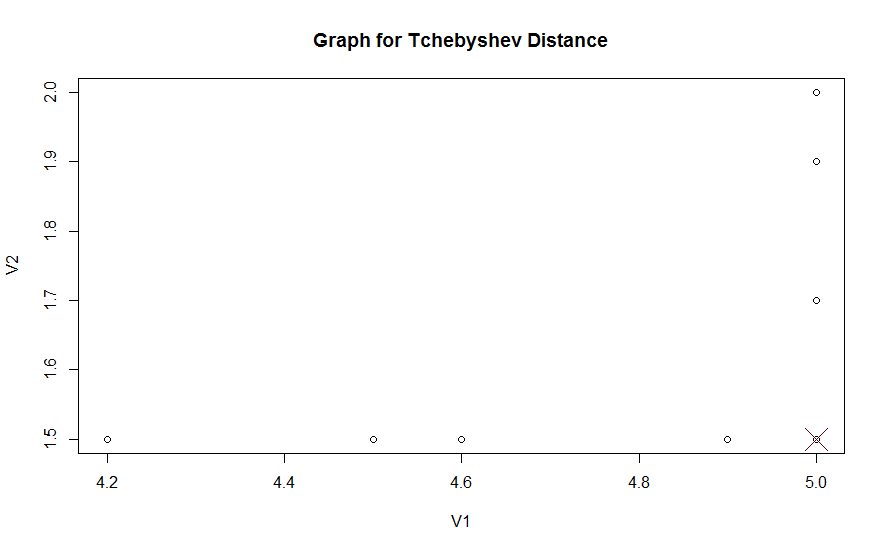
\includegraphics[scale=.5]{resources/tchebyshev.png}
					\caption{The plot for Tchebyshev Distance}
				\end{center}
			\end{figure}

			\newpage
			\textbf{\large Cosine Distance} \\

				Using Cosine Distance as opposde to cosine similarity.
\begin{verbatim}
> cos1 <- cbind(vals,cosdist)
> cos2<-head(cos1[order(cosdist),],10)
> plot(cos2[["V1"]],cos2[["V2"]],xlab="V1",ylab="V2",
+				main="Graph for Cosine Distance")
> points(5,1.5,type="b",pch=4,col="#660000",cex=3)

\end{verbatim}
			\begin{figure}[H]
				\begin{center}
					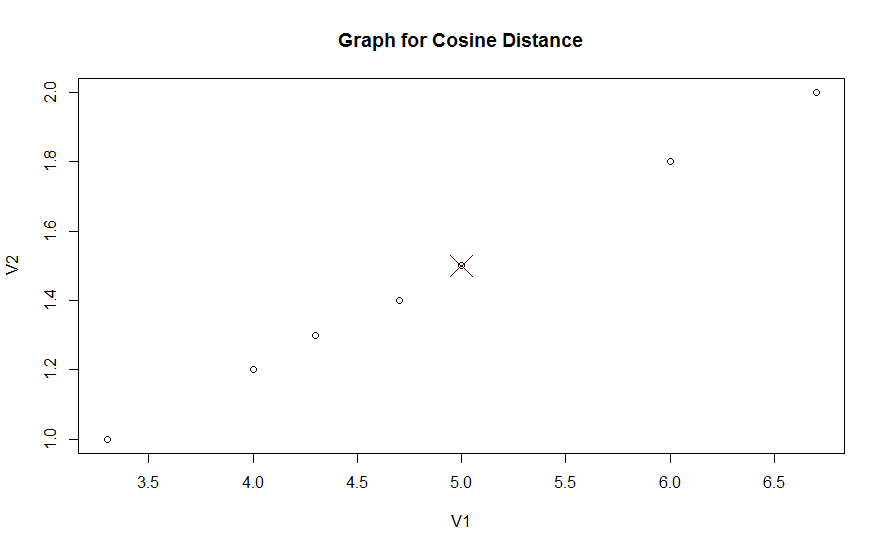
\includegraphics[scale=.5]{resources/cosine.png}
					\caption{The plot for Cosine Distance}
				\end{center}
			\end{figure}

			\newpage
			\textbf{\large Manhattan Distance} \\

\begin{verbatim}
> manh1 <- cbind(vals,manhattan)
> manh2<-head(manh1[order(manhattan),],10)
> plot(manh2[["V1"]],manh2[["V2"]],xlab="V1",ylab="V2"
+	,main="Graph for Manhattan Distance")
> points(5,1.5,type="b",pch=4,col="#660000",cex=3)

\end{verbatim}
			\begin{figure}[H]
				\begin{center}
					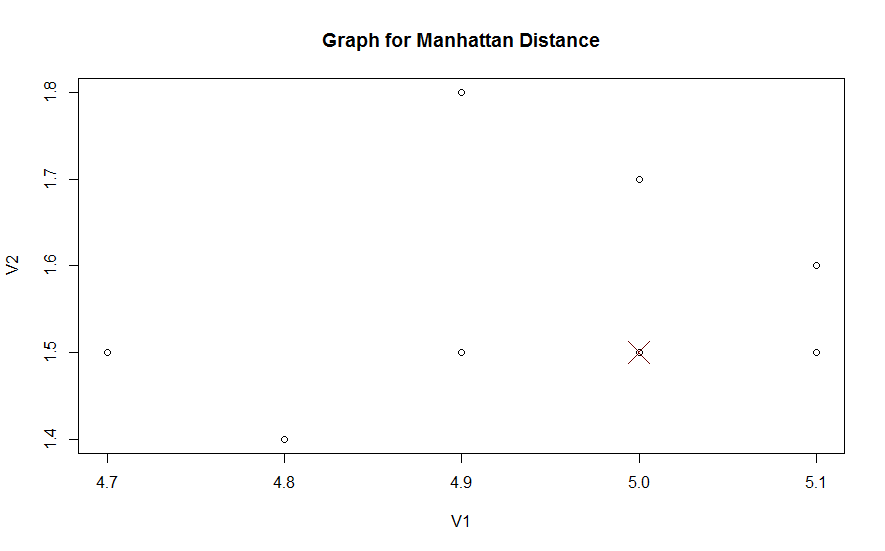
\includegraphics[scale=.5]{resources/manhattan.png}
					\caption{The plot for Manhattan Distance}
				\end{center}
			\end{figure}


			\newpage
			\textbf{\large Euclidean Distance} \\

\begin{verbatim}
> euc1 <- cbind(vals,euclid)
> euc2<-head(euc1[order(euclid),],10)
> plot(euc2[["V1"]],euc2[["V2"]],xlab="V1",ylab="V2"
+					,main="Graph for Euclidean Distance")
> points(5,1.5,type="b",pch=4,col="#660000",cex=3)

\end{verbatim}
			\begin{figure}[H]
				\begin{center}
					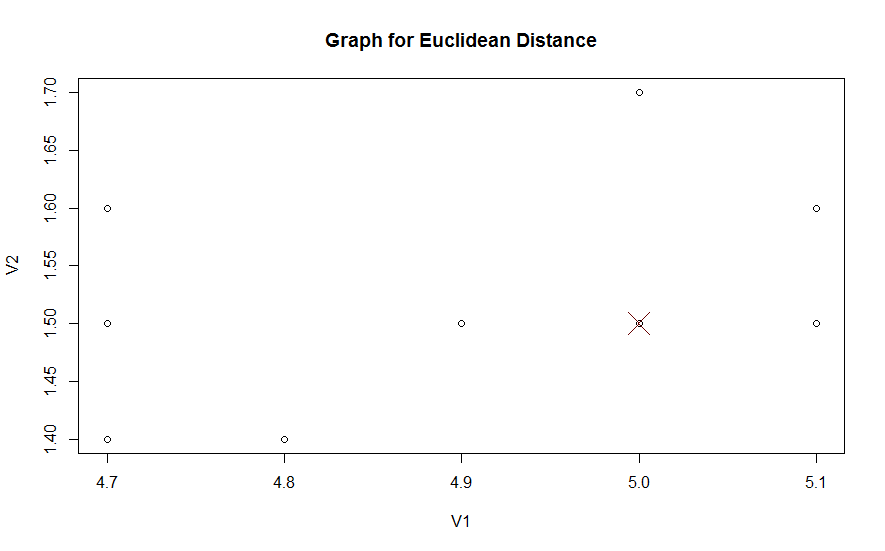
\includegraphics[scale=.5]{resources/euclidean.png}
					\caption{The plot for Manhattan Distance}
				\end{center}
			\end{figure}


			\end{enumerate}
	\end{enumerate}
\end{document}		
